\documentclass[tikz]{standalone}
\usepackage{physics}
\usetikzlibrary{arrows.meta,decorations.pathmorphing,patterns,decorations.pathreplacing}

\begin{document}
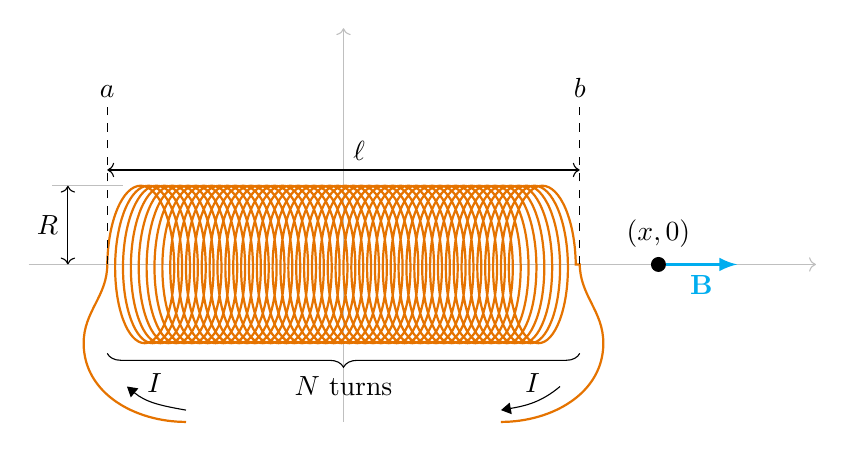
\begin{tikzpicture}
  % axis lines
  \draw[->,lightgray] (-4,0) -- (6,0);
  \draw[->,lightgray] (0,-2) -- (0,3);

  % solenoid
  \draw[thick,orange!90!black,decoration={aspect=0.4, segment length=1mm, amplitude=10mm,coil,post length=0mm},decorate] (-3,0) -- (3,0);
  %\draw [thin, blue] plot [smooth, tension=1] coordinates {(-3,0) (-3.05,-0.25) (-3.3,-0.9) (-2.8,-2) (-1.5,-2.2)};
  \draw [thick,orange!90!black] (-3,0) to [out=270,in=90] (-3.3,-1) to [] [out=270,in=180] (-2,-2) ;
  \draw [thick,orange!90!black] (3,0.014) to [out=270,in=90] (3.3,-1) to [] [out=270,in=0] (2,-2) ;


  % Point
  \node[circle,draw,fill=black,inner sep=0,minimum size=5pt] (p) at (4,0){};
  \node[anchor=south] at (p.north){$(x,0)$};

  % Dashed lines
  \draw[dashed] (3,0) -- node[pos=1,anchor=south]{$b$} (3,2);
  \draw[dashed] (-3,0) -- node[pos=1,anchor=south]{$a$} (-3,2);

  % Distances and data
  \draw[<->] (-3,1.2) --node[anchor=south west]{$\ell$} (3,1.2);
  \draw [decorate,decoration={brace,amplitude=5pt},xshift=0pt,yshift=2pt] (3,-1.2) -- (-3,-1.2) node [black,midway,anchor=north,yshift=-5pt] {$N$ turns};
  \draw[lightgray] (-3.7,1) -- (-2.8,1);
  \draw[<->] (-3.5,0) --node[anchor=east]{$R$} (-3.5,1);
  \draw[-Triangle] (-2,-1.85) to [out=170,in=320] node[anchor=south]{$I$} (-2.75,-1.55);
  \draw[Triangle-] (2,-1.85) to [out=10,in=220] node[anchor=south]{$I$} (2.75,-1.55);

  % Magnetic field
  \draw[very thick,-latex,cyan] (p.east) -- node[anchor=north]{$\vb{B}$} (5,0);
\end{tikzpicture}
\end{document}
